\documentclass[fsharpNotes.tex]{subfiles}
\graphicspath{ {./figures/} }

\begin{document}
\chapter{Values, Functions, and Statements}
\label{chap:let}
%
\abstract[figures/valuesFunctionsNStatements]{
In the previous chapter, you got an introduction to the fundamental concepts of booleans, numbers, characters, and strings, how to perform calculations with them, and some of the limitations they have on the computer. This allows us to perform simple calculations as if the computer was an advanced pocket calculator. In this chapter, we will look at how we can:
  \begin{itemize}
  \item Make assign values to names to make programs that are easier to read and write.
  \item Organise lines of code in functions, to make the same line reusable, and to make programs shorter, and easier to understand.
  \item Use operators as functions.
  \item Conditionally execute code.
  \item How we can simulate the computer's execution of code by tracing-by-hand, to improve our understanding of, how it interprets the code, we write, and to find errors.
  \end{itemize}
  Examples of problems, you can solve, after having read this chapter are:
  \begin{itemize}
  \item Write a function that given the parameters $a$ and $b$ in $f(x) = ax+b$, find the value of $x$ when $f(x)=0$.
  \item 
  \end{itemize}
}

In this chapter, we will see how we can bind expressions to identifiers either as new constants, functions, or operators, how this saves time when building large programs, and how this makes programs easier to read and debug. As an example, consider the following problem,
\begin{task}
  For given set constants $a$, $b$, and $c$, solve for $x$ in
  \begin{equation}
  a x^2+bx+c = 0
\end{equation}
\end{task}
To solve for $x$ we use the quadratic formula from elementary algebra,
\begin{equation}
  x = \frac{-b\pm\sqrt{b^2-4ac}}{2a},
\end{equation}
which gives the general solution for any values of the coefficients. Here, we will assume a positive discriminant, $b^2-4ac>0$. In order to write a program where the code may be reused later, we define a function
\begin{quote}
  \lstinline!discriminant : float -> float -> float -> float!
\end{quote}
that is, a function that takes 3 arguments, \lstinline!a!, \lstinline!b!, and \lstinline!c!, and calculates the discriminant. Likewise, we will define
\begin{quote}
  \lstinline!positiveSolution : float -> float -> float -> float!
\end{quote}
and
\begin{quote}
  \lstinline!negativeSolution : float -> float -> float -> float!
\end{quote}
that also take the polynomial's coefficients as arguments and calculate the solution corresponding to choosing the positive and negative sign for $\pm$ in the equation. Details on function definition is given in \Cref{sec:functions}. Our solution thus looks like \Cref{identifiersExample}.
%
\fs{identifiersExample}{Finding roots for quadratic equations using function name binding.}
%
Here, we have further defined names of values \lstinline!a!, \lstinline!b!, and \lstinline!c! which are used as inputs to our functions, and the results of function application are bound to the names \lstinline!d!, \lstinline!xn!, and \lstinline!xp!. The names of functions and values given here are examples of identifiers, and with these, we may reuse the quadratic formulas and calculated values later, while avoiding possible typing mistakes and reducing the amount of code that needs to be debugged.

The use of identifiers is central in programming. For F\#, not to be confused with built-in functionality, identifiers must follow a specific set of rules: 
\begin{description} 
\item[Identifier]\idxs{identifier}~\\[-5mm]
  \begin{itemize}
  \item Identifiers are used as names for values, functions, types etc.
  \item They must start with a Unicode letter or underscore '\_', but can be followed by zero or more letters, digits, and a range of special characters except for SP, LF, and CR (space, line feed, and carriage return). See \Cref{sec:unicode} for more on codepoints that represent letters. 
  \item They can also be a sequence of identifiers separated by a period.
  \item They cannot be keywords, see \Cref{tab:keywords}.
  \end{itemize}
\end{description}
\begin{table}
  \centering
  \rowcolors{2}{oddRowColor}{evenRowColor}
  \begin{tabularx}{\textwidth}{|l|>{\raggedright\arraybackslash}X|}
    \hline
    \rowcolor{headerRowColor} Type & Keyword\\
    \hline
  Regular 
  &\mbox{\lstinline{abstract},} \mbox{\lstinline{and},} \mbox{\lstinline{as},} \mbox{\lstinline{assert},} \mbox{\lstinline{base},} \mbox{\lstinline{begin},} \mbox{\lstinline{class},} \mbox{\lstinline{default},} \mbox{\lstinline{delegate},} \mbox{\lstinline{do},} \mbox{\lstinline{done},} \mbox{\lstinline{downcast},} \mbox{\lstinline{downto},} \mbox{\lstinline{elif},} \mbox{\lstinline{else},} \mbox{\lstinline{end},} \mbox{\lstinline{exception},} \mbox{\lstinline{extern},} \mbox{\lstinline{false},} \mbox{\lstinline{finally},} \mbox{\lstinline{for},} \mbox{\lstinline{fun},} \mbox{\lstinline{function},} \mbox{\lstinline{global},} \mbox{\lstinline{if},} \mbox{\lstinline{in},} \mbox{\lstinline{inherit},} \mbox{\lstinline{inline},} \mbox{\lstinline{interface},} \mbox{\lstinline{internal},} \mbox{\lstinline{lazy},} \mbox{\lstinline{let},} \mbox{\lstinline{match},} \mbox{\lstinline{member},} \mbox{\lstinline{module},} \mbox{\lstinline{mutable},} \mbox{\lstinline{namespace},} \mbox{\lstinline{new},} \mbox{\lstinline{null},} \mbox{\lstinline{of},} \mbox{\lstinline{open},} \mbox{\lstinline{or},} \mbox{\lstinline{override},} \mbox{\lstinline{private},} \mbox{\lstinline{public},} \mbox{\lstinline{rec},} \mbox{\lstinline{return},} \mbox{\lstinline{sig},} \mbox{\lstinline{static},} \mbox{\lstinline{struct},} \mbox{\lstinline{then},} \mbox{\lstinline{to},} \mbox{\lstinline{true},} \mbox{\lstinline{try},} \mbox{\lstinline{type},} \mbox{\lstinline{upcast},} \mbox{\lstinline{use},} \mbox{\lstinline{val},} \mbox{\lstinline{void},} \mbox{\lstinline{when},} \mbox{\lstinline{while},} \mbox{\lstinline{with},} and \mbox{\lstinline{yield}.}\\
 Reserved
 & \mbox{\lstinline{atomic},} \mbox{\lstinline{break},} \mbox{\lstinline{checked},} \mbox{\lstinline{component},} \mbox{\lstinline{const},} \mbox{\lstinline{constraint},} \mbox{\lstinline{constructor},} \mbox{\lstinline{continue},} \mbox{\lstinline{eager},} \mbox{\lstinline{fixed},} \mbox{\lstinline{fori},} \mbox{\lstinline{functor},} \mbox{\lstinline{include},} \mbox{\lstinline{measure},} \mbox{\lstinline{method},} \mbox{\lstinline{mixin},} \mbox{\lstinline{object},} \mbox{\lstinline{parallel},} \mbox{\lstinline{params},} \mbox{\lstinline{process},} \mbox{\lstinline{protected},} \mbox{\lstinline{pure},} \mbox{\lstinline{recursive},} \mbox{\lstinline{sealed},} \mbox{\lstinline{tailcall},} \mbox{\lstinline{trait},} \mbox{\lstinline{virtual},} and \mbox{\lstinline{volatile}.}\\
 Symbolic
 & \mbox{\lstinline{let!},} \mbox{\lstinline{use!},} \mbox{\lstinline{do!},} \mbox{\lstinline{yield!},} \mbox{\lstinline{return!},} \mbox{\lstinline{|},} \mbox{\lstinline{->},} \mbox{\lstinline{<-},} \mbox{\lstinline{.},} \mbox{\lstinline{:},} \mbox{\lstinline{(},} \mbox{\lstinline{)},} \mbox{\lstinline{[},} \mbox{\lstinline{]},} \mbox{\lstinline{[<},} \mbox{\lstinline{>]},} \mbox{\lstinline{[|},} \mbox{\lstinline{|]},} \mbox{\lstinline{\{},} \mbox{\lstinline{\}},} \mbox{\lstinline{'},} \mbox{\lstinline{#},} \mbox{\lstinline{:?>},} \mbox{\lstinline{:?},} \mbox{\lstinline{:>},} \mbox{\lstinline{..},} \mbox{\lstinline{::},} \mbox{\lstinline{:=},} \mbox{\lstinline{;;},} \mbox{\lstinline{;},} \mbox{\lstinline{=},} \mbox{\lstinline{_},} \mbox{\lstinline{?},} \mbox{\lstinline{??},} \mbox{\lstinline{(*)},} \mbox{\lstinline{<@},} \mbox{\lstinline{@>},} \mbox{\lstinline{<@@},} and \mbox{\lstinline{@@>}.} \\
 Reserved symbolic
 &\mbox{\lstinline{\~}} and \mbox{\lstinline{`}}\\
    \hline
  \end{tabularx}
  \caption{Table of (possibly future) \emph{keywords}\idxss{keyword} and symbolic keywords in F\#.}
  \label{tab:keywords}
\end{table}
Examples of identifiers are: \lstinline{a}, \lstinline{theCharacter9}, \lstinline{Next_Word}, \lstinline{_tok}, and \lstinline{f.sharp.rocks}.  Since programmers often work in a multilingual environment dominated by the English language it is advisable to \advice{restrict identifiers to use letters from the English alphabet, numbers, periods, and '\_'.}  However, the number of possible identifiers is enormous. The full definition refers to the Unicode general categories described in Appendix~\ref{sec:unicode}, and there are currently 19.345 possible Unicode code points in the latter category and 2.245 possible Unicode code points in the special character category.

Identifiers may be used to carry information about their intended content and use, and a careful selection of identifiers can aid programmers to communicate thoughts about the code. Thus, identifiers are often a word or several concatenated words conveying some relevant meaning. For example, in the function definition \lstinline{let discriminant a b c = b ** 2.0 - 4.0 * a * c}, the function identifier has been chosen to be \lstinline{discriminant}. F\# places no special significance on the word 'discriminant', and the program would work exactly the same had the function been called \lstinline{let f a b c = b ** 2.0 - 4.0 * a * c}. However, to programmers, the word 'discriminant' informs us of the intended role of the function and thus is much preferred. This is a general principle: \advice{identifier names should be chosen to reflect their semantic value.}. The arguments \lstinline{a}, \lstinline{b}, and \lstinline{c} are short, but adheres to a textbook tradition of elementary algebra. Again, we might as well have used, \lstinline{let discriminant c a b = a ** 2.0 - 4.0 * c * b}, which is semantically identical to the original expression, but due to tradition, this would confuse most readers of the code. Thus, \advice{identifier names should be chosen consistently with the readers' traditions.} Finally, identifiers are often concatenations of words, as \lstinline{positiveSolution} in \Cref{identifiersExample}. Concatenations can be difficult to read. Without the capitalization of the second word, we would have had \lstinline{positivesolution}. This is readable at most times but takes longer time to understand in general. Typical solutions are to use a separator, such as \lstinline{positive_solution}, \idx{lower camel case} also known as \idx{mixed case} as in the example \lstinline{positiveSolution}, and \idx{upper camel case} also known as \idx{pascal case} as \lstinline{PositiveSolution}. In this book, we use the lower camel case except where F\# requires a capital first letter. Again, the choice does not influence what a program does, only how readable it is to a fellow programmer. The important part is that \advice{identifier names consisting of concatenated words are often preferred over names with few characters, and concatenation should be emphasized, e.g., by camel casing.} Choosing the length of identifier names is a balancing act, since when working with large programs, very long identifier names can be tiresome to write, and a common practice is that the length of identifier names is proportional to the complexity of the program. I.e., complex programs use long names, simple programs use short names. What is complex and what is simple is naturally in the eye of the beholder, but when you program, remember that a future reader of the program most likely has not had time to work with the problem as long as the programmer, thus \advice{choose identifier names as if you were to explain the meaning of a program to a knowledgeable outsider.}

Another key concept in F\# is expressions. An expression can be a mathematical expression, such as $3*5$, a function application, such as $f 3$, and many other things. Central in this chapter is the binding of values and functions to identifiers, which is done with the keyword \keyword{let}, e.g., \lstinline!let a = 1.0!.

Expressions are the main workhorse of F\# and have an enormous variety in how they may be written. We will in this book gradually work through some of the more important facets.
\begin{description} 
\item[Expressions]\idxs{expression}~\\[-5mm]
  \begin{itemize}
  \item An Expression is a computation such as \lstinline{3 * 5}.
  \item They can be value bindings between identifiers and expressions that evaluate to a value or a function, see \Cref{sec:values,sec:functions}.
  \item They can be \lstinline{do}-bindings that produce side-effects and whose results are ignored, see \Cref{sec:functions} 
  \item They can be assignments to variables, see \Cref{sec:values}.
  \item They can be a sequence of expressions separated with the \idx[;@\lstinline{;}]{\lexeme{;}} lexeme.
  \item They can be annotated with a type by using the \idx[:@\lstinline{:}]{\lexeme{:}} lexeme.
  \end{itemize}
\end{description}

Before we begin a deeper discussion on bindings, note that F\#  adheres to two different syntaxes: \idx[verbose syntax]{verbose} and \idx[lightweight syntax]{lightweight}. In the verbose syntax, newlines and whitespaces are generally ignored, while in lightweight syntax, certain keywords and lexemes may be replaced by newlines and whitespaces. The lightweight syntax is the most common and will be used in this book.

\section{Value Bindings}
\label{sec:values}
Binding identifiers to literals, or expressions that are evaluated to be values, is called \idx{value-binding}, and examples are \lstinline!let a = 3.0! and \lstinline!let b = cos 0.9!. Value bindings have the following syntax:
%
\begin{verbatimwrite}{\ebnf/valueBindings.ebnf}
let <*valueIdent*> = <*bodyExpr*>
\end{verbatimwrite}
\syntax{\ebnf/valueBindings.ebnf}{Value binding expression.}
%
The \idx[let@\lstinline{let}]{\keyword{let}} keyword binds a value-identifier with an expression. The above notation means that \lstinline[language=syntax]{<*valueIdent*>} is to be replaced with a name and \lstinline[language=syntax]{<*bodyExpr*>} with an expression that evaluates to a value. The binding \emph{is} available in later lines until the end of the scope it is defined in.

The value identifier is annotated with a type by using the \idx[:@\lstinline{:}]{\lexeme{:}} lexeme followed by the name of a type, e.g., \lstinline{int}. The \idx[\_@\lstinline{_}]{\lexeme{\_}} lexeme may be used as a value-identifier. This lexeme is called the \idx{wildcard pattern}, and for value-bindings it means that \lstinline[language=syntax]{<*bodyExpr*>} is evaluated, but the result is discarded. See \Cref{chap:patterns} for more details on patterns.

For example, letting the identifier \lstinline!p! be bound to the value \lstinline!2.0! and using it in an expression is done as shown in \Cref{letValueLightWeight}.
%
\fs{letValueLightWeight}{Lightweight syntax does not require the \keyword{in} keyword, but the expression must be aligned with the \keyword{let} keyword.}
%
Note that the expression \lstinline{3.0 ** p} must be put in parentheses here, to force F\# to \emph{first} calculate the result of the expression and \emph{then} give it to \lstinline{printfn} to be printed on the screen. The same expression in interactive mode will also show with the inferred types, as shown in \Cref{letValueLightWeightTypes}.
%
\fsOutput{letValueLightWeightTypes}{Interactive mode also outputs inferred types.}
%
By the \keyword{val} keyword in the line \lstinline!val p : float = 2.0!, we see that \lstinline!p! is inferred to be of type \lstinline!float! and bound to the value \lstinline!2.0!. The inference is based on the type of the right-hand-side which is \lstinline!float!.  Identifiers may be defined to have a type using the \lexeme{:} lexeme, but the types on the left-hand-side and right-hand-side of the \lexeme{=} lexeme must be identical. Mixing types gives an error, as shown in \Cref{letValueTypeError}.
%
\fs{letValueTypeError}{Binding error due to type mismatch.}
% \begin{lstlisting}[language=fsharp,caption={fsharpi, binding error due to type mismatch.}]
%   > let a : float = 3;;
%
%   let a : float = 3;;
%   ----------------^
%
% /Users/sporring/repositories/fsharpNotes/stdin(50,17): error FS0001: This expression was expected to have type
%     float    
% but here has type
%     int    
% \end{lstlisting}
Here, the left-hand side is defined to be an identifier of type float, while the right-hand side is a literal of type integer.

%An expression can be a sequence of expressions separated by the lexeme \lexeme{;}, see \Cref{letValueSequence}.
%%
%\fs{letValueSequence}{A value-binding for a sequence of expressions.}
%%
%The lightweight syntax automatically inserts the \lexeme{;} lexeme at newlines, hence using the lightweight syntax, the above is the same as shown in \Cref{letValueSequenceLightWeight}.
%%
%\fs{letValueSequenceLightWeight}{A value-binding for a sequence using lightweight syntax.}
%%

A key concept of programming is \idx{scope}. When F\# seeks the value bound to a name, it looks left and upward in the program text for its \keyword{let}-binding in the present or higher scopes.
% , see \Cref{letValueScopeLower} for an example.
This is called \idx{lexical scope}.
%%
%\fs{letValueScopeLower}{Redefining identifiers is allowed in lower scopes.}
%%
Some special bindings are mutable, that is, they can change over time in which case F\# uses the \idx{dynamic scope}. This will be discussed in \Cref{sec:mutableValues}.

Scopes are given levels, and scopes may be nested, where the nested scope has a level one lower than its parent.\jon{Drawings would be good to describe scope} F\# distinguishes between the top and lower levels, and at the top level in the lightweight syntax, redefining values is not allowed, as shown in \Cref{letValueScopeLowerError}.
%
\fs{letValueScopeLowerError}{Redefining identifiers is not allowed in lightweight syntax at top level.}
%
%But using \keyword{begin} and \keyword{end} keywords, we create a \idx{block} which acts as a \idx{nested scope}, and then redefining is allowed, e.g.,
% %
% \fs{letValueScopeBlockAlternative2}{A block has lower scope level, and rebinding is allowed.}
% %
% It is said that the second binding \idx{overshadows} the first.
% Alternatively, we may use parentheses to create a block, e.g.,
However, using parentheses, we create a \idx{code block}, i.e., a \idx{nested scope}, as demonstrated in \Cref{letValueScopeBlockAlternative3}.
%
\fs{letValueScopeBlockAlternative3}{A block may be created using parentheses.}
%
In lower scope-levels, redefining is allowed but \advice{avoid reusing names unless it's in a deeper scope.} Inside the block in \Cref{letValueScopeBlockAlternative3} we used indentation, which is good practice, but not required here.

Defining blocks is used for controlling the extent of a lexical scope of bindings. For example, bindings inside a nested scope are not available outside, as shown in \Cref{letValueScopeNestedScope}.
%
\fs{letValueScopeNestedScope}{Bindings inside a scope are not available outside.}
%
Nesting is a natural part of structuring code, e.g., through function definitions to be discussed in \Cref{sec:functions} and flow control structures to be discussed in \Cref{chap:flow}. Blocking code by nesting is a key concept for making robust code that is easy to use by others, without the user necessarily needing to know the details of the inner workings of a block of code.


%adding a second \lstinline!printfn! statement, as in \Cref{letValueScopeBlockProblem},
%will print the value 4, last bound to the identifier \lstinline!p!, since F\# interprets the above as \lstinline!let p = 3 in let p = 4 in (printfn "%A" p; printfn "%A" p)!. %
%%
%\fs{letValueScopeBlockProblem}{Overshadowing hides the first binding.}
%%
%Had we intended to print the two different values of \lstinline!p!, then we should have created a block as in \Cref{letValueScopeBlock}.
%%
%\fs{letValueScopeBlock}{Blocks allow for the return to the previous scope.}
%%
%%Here, the lexical scope of \lstinline!let p = 4! is for the nested scope, which ends at \lexeme{)}, returning to the lexical scope of \lstinline!let p = 3 in ...!. %Alternatively, the \keyword{begin} and \keyword{end} keywords could equally have been used.
%\fs{letValueScopeBlockAlternative}{}

\section{Function Bindings}
\label{sec:functions}
A function is a mapping between an input and output domain, as illustrated in Figure~\Cref{fig:functions}.
\begin{figure}
  \centering
  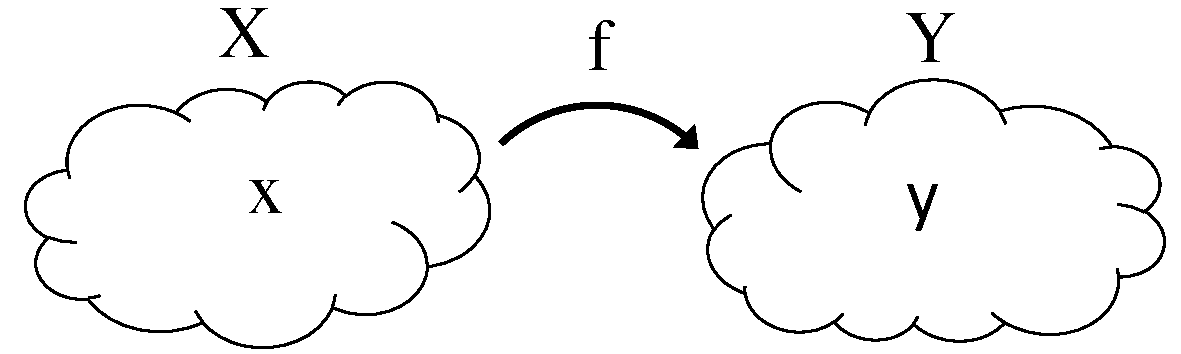
\includegraphics[width=0.6\linewidth]{functions}
  \caption{A function $f:X\rightarrow Y$ is a mapping between two domains, such that $f(x)=y,\, x\in X,\, y\in Y$.}
  \label{fig:functions}
\end{figure}
A key advantage of using functions when programming is that they encapsulate\idxss{encapsulation} code into smaller units, that may be reused and are easier to find errors in. F\# is a functional-first programming language and offers a number of alternative methods for specifying parameters, which will be discussed in this section. Binding identifiers to functions follows a syntax similar to value-binding,
%
\begin{verbatimwrite}{\ebnf/functionBindings.ebnf}
let <*ident*> (*<*arg*> {*<*arg*>*}*) |* () =
  <*expr*>
\end{verbatimwrite}
\syntax{\ebnf/functionBindings.ebnf}{Function binding expression}
%
Here \lstinline[language=syntax]{<*ident*>} is an identifier and is the name of the function, \lstinline[language=syntax]{<*arg*>} is zero or more identifiers, that bind to the value used when calling the function, and which is to be used in the \idx[function body]{body} of the function, the expression \lstinline[language=syntax]{<*expr*>}. The \lstinline[language=syntax]{|*} notation denotes a choice, i.e., either that on the left-hand side or that on the right-hand side. Thus \lstinline{let f x = x * x} and \lstinline{let f () = 3} are valid function bindings, but \lstinline{let f = 3} would be a value binding, not a function binding. The arguments and the function may be annotated with a type, in which case for arguments we write
%
\begin{verbatimwrite}{\ebnf/functionBindingsAnnotated.ebnf}
let <*ident*> (*(<*arg*> : <*type*>) {*(<*arg*> : <*type*>)*} : <*type*>*) |* (*() : <*type*>*) =
  <*expr*>
\end{verbatimwrite}
\syntax{\ebnf/functionBindingsAnnotated.ebnf}{Function binding expression}
%
where \lstinline[language=syntax]{<*type*>} is a name of an existing type. The argument types are given in parentheses, and the return type is given last. 

Functions are a key concept in F\#, and in this chapter, we will discuss the very basics. Recursive functions will be discussed in \Cref{chap:flow} and higher-order functions in \Cref{chap:higherOrderFunctions}.

The function's body can be placed either on the same line as the \keyword{let}-keyword or on the following lines using indentation. An example of defining a function and using it in interactive mode is shown in \Cref{letFunction}.
%
\fsOutput{letFunction}{An example of a binding of an identifier and a function.}
%
Here we see that the function is interpreted to have the type \lstinline!val sum : x:float -> y:float -> float!. The \lexeme{->} lexeme means a mapping between sets, in this case, floats. The function is also a higher-order function, to be discussed in detail below, and here it suffices to think of \lstinline!sum! as a function that takes 2 floats as arguments and returns a float.
%, that \lexeme{->} associates to the right, hence \lstinline!x:float -> y:float -> float! is equivalent to \lstinline!x:float -> (y:float -> float)! and thus, \lstinline!sum x! is a function, which gives a function

Not all types need to be declared, just a sufficient number for F\# to be able to infer the types for the full statement. For the example, one is sufficient, and we could just have declared the type of the result, as in \Cref{letFunctionAlterantive}.
%
\fsCode{letFunctionAlterantive}{letFunctionAlterantive}{Not every type needs to be declared.}{}
%
Or even just one of the arguments, as in \Cref{letFunctionAlterantive2}.
%
\fsCode{letFunctionAlterantive2}{letFunctionAlterantive2}{Just one type is often enough for F\# to infer the rest.}{}
%
In both cases, since the \lstinline|+| \idx{operator} is only defined for \idx[operand]{operands} of the same type, declaring the type of either arguments or result implies the type of the remainder.
% As for values, lightweight syntax automatically inserts the keyword \keyword{in} and the lexeme \lexeme{;}, as shown in \Cref{letFunctionLightWeight}.
% %
% \fs{letFunctionLightWeight}{Lightweight syntax for function definitions.}
% %

Arguments need not always be inferred to types, but may be of the generic type when \idx{type safety} is ensured, as shown in \Cref{functionDeclarationGeneric}.
%
\fsOutput{functionDeclarationGeneric}{Type safety implies that a function will work for any type.}
%
Here, the function \lstinline{second} does not use the first argument \lstinline{x}, which therefore can be of any type, and which F\#, therefore, calls \lstinline{'a}. The type of the second element, \lstinline{y}, can also be of any type and not necessarily the same as \lstinline!x!, so it is called \lstinline!'b!. Finally, the result is the same type as \lstinline!y!, whatever it is. This is an example of a \idx{generic function}, since it will work on any type.

A function may contain a sequence of expressions but must return a value. E.g., the quadratic formula may be written as shown in \Cref{identifiersExampleAdvance}. 
%
\fs{identifiersExampleAdvance}{A function may contain sequences of expressions.}
%
Here, we use a set of nested scopes. In the scope of the function \lstinline{solution} there are further two functions defined, each with their own scope, which F\# identifies by the level of indentation. The amount of space used for indentation does not matter, but all lines in the same scope must use the same amount. The scope ends before the first line with the previous indentation or none. Notice how the last expression is not bound to an identifier but is the result of the function, i.e., in contrast to many other languages, F\# does not have an explicit keyword for returning values but requires a final expression, which will be returned to the caller of the function. Note also that since the function \lstinline!discriminant! is defined in the nested scope of \lstinline!solution!, and because the scope ends before \lstinline!let a = 1.0!, the function \lstinline!discriminant! cannot be called outside \lstinline!solution!.

\idx[lexical scope]{Lexical scope} and function definitions can be a cause of confusion, as the following example in \Cref{lexicalScopeNFunction} shows.\jon{Add a drawing or possibly a spell-out of lexical scope here.}
%
\fs{lexicalScopeNFunction}{Lexical scope means that $f(z) = 3x$ and not $4x$ at the time of calling.}
%
Here, the value-binding for \lstinline!a! is redefined after it has been used to define a helper function \lstinline!f!. So which value of \lstinline!a! is used when we later apply \lstinline!f! to an argument? To resolve the confusion, remember that value-binding is lexically defined, i.e., the binding \lstinline!let f z = a * z! uses the value of \lstinline!a! as it is defined by the ordering of the lines in the script, not dynamically by when \lstinline!f! was called. Hence, \advice{think of lexical scope as substitution of an identifier with its value or function immediately at the place of definition.} Since \lstinline!a! and \lstinline!3.0! are synonymous in the first lines of the program, the function \lstinline!f! is really defined as \lstinline!let f z = 3.0 * z!.

Functions do not need a name, but may be declared as an \idx[anonymous functions]{anonymous function}\label{page:anonymousFunction} using the \idx[fun@\lstinline{fun}]{\keyword{fun}} keyword and the \idx[->@\lstinline{->}]{\lexeme{->}} lexeme, as shown in \Cref{functionDeclarationAnonymous}.
%
\fs{functionDeclarationAnonymous}{Anonymous functions are functions as values.}
%
Here, a name is bound to an anonymous function which returns the first of two arguments. The difference to \lstinline!let first x y = x! is that anonymous functions may be treated as values, meaning that they may be used as arguments to other functions and the new values may be reassigned to their identifiers when mutable, as will be discussed in \Cref{sec:mutableValues}. A common use of anonymous functions is as arguments to other functions, as demonstrated in \Cref{functionDeclarationAnonymousAdvanced}.
%
\fs{functionDeclarationAnonymousAdvanced}{Anonymous functions are often used as arguments for other functions.}
%
Note that here \lstinline!apply! is given 3 arguments: the function \lstinline!mul! and 2 integers. It is not given the result of \lstinline!mul 3 6!, since that would not match the definition of \lstinline!apply!. \advice{Anonymous functions and functions as arguments are powerful concepts but tend to make programs harder to read, and their use should be limited.}

\label{page:piping}
The result of one function is often used as an argument of another. This is function composition, and an example is shown in \Cref{functionComposition}.
%
\fs{functionComposition}{Composing functions using intermediate bindings.}
%
In the example we combine two functions \lstinline{f} and \lstinline{g} by storing the result of \lstinline{f 2} in \lstinline{a} and using that as argument of \lstinline{g}. This is the same as \lstinline{g (f 2)}, and in the later case, the compile creates a temporary value for \lstinline{f 2}. Such compositions are so common in F\# that a special set of operators has been invented, called the \idx{piping} operators: \idx[{|>}@\lstinline{|>}]{\lexeme{|>}} and \idx[{<|}@\lstinline{<|}]{\lexeme{<|}}. They are used as demonstrated in \Cref{functionPiping}.
%
\fs{functionPiping}{Composing functions by piping.}
%
The example shows regular composition, left-to-right, and right-to-left piping. The word piping is a pictorial description of data as if it were flowing through pipes, where functions are connection points of pipes distributing data in a network. The three expressions in \Cref{functionPiping} perform the same calculation. The left-to-right piping in line~\ref{functionPipingLeftToRight} corresponds to the left-to-right reading direction, i.e., the value \lstinline{2} is used as argument to \lstinline{f}, and the result is used as argument to \lstinline{g}. In contrast, right-to-left piping in line~\ref{functionPipingRightToLeft} has the order of arithmetic composition as line~\ref{functionPipingComposition}. Unfortunately, since the piping operators are left-associative, without the parenthesis in line~\ref{functionPipingRightToLeft} \mbox{\lstinline{g <| f <| 2}}, F\# would read the expression as \lstinline{(g <| f) <| 2}. That would have been an error since \lstinline{g} takes an integer as an argument, not a function. F\# can also define composition on a function level. Further discussion on this is deferred to \Cref{chap:higherOrderFunctions}.

%% Jon 20220828: Tuple piping, should it be introduced later?
%The piping operator comes in four variants: \lexeme{||>}, \lexeme{<||}, \lexeme{|||>}, and \lexeme{<|||}. These allow for piping between pairs and triples to functions of 2 an%d 3 arguments, see \Cref{functionTuplePiping} for an example.
%%
%\fs{functionTuplePiping}{Tuples can be piped to functions of more than one argument.}
%%
%The example demonstrates right-to-left piping, left-to-right works analogously.\jon{Tuples have not yet been introduced!}

A \idx{procedure} is a generalization of the concept of functions, and in contrast to functions, procedures need not return values. This is demonstrated in \Cref{procedure}.
%
\fs{procedure}{A procedure is a function that has no return value, and in F\# returns \lexeme{()}.}
%
In F\#, this is automatically given the unit type as the return value. Procedural thinking is useful for \idx{encapsulation} of scripts, but is prone to \idx[side-effect]{side-effects}. 
%An example, we've already seen is the \lstinline{printfn}, which is used to print text on the console but does not return a value. Coincidentally, since the console is a state, printing to it is a side-effect. Above we examined 
%\begin{fse}
%   let updateFactor factor = 
%    factor := 2
%\end{fse}
%\fsCode{mutableAssignReturnSideEffectStump}{mutableAssignReturnSideEffectStump}{}{}
%which also does not have a return value. 
For this reason, it is advised to \advice{prefer functions over procedures.}  More on side-effects in \Cref{sec:mutableValues}.

In F\#, functions (and procedures) are \idx[first-class citizenship]{first-class citizens}, which means that functions are values: They may be passed as arguments, returned from a function, and bound to a name. For first-class citizens, the name it is bound to does not carry significance to the language, as, e.g., illustrated with the use of anonymous functions. Technically, a function is stored as a \idx{closure}. A closure is a description of the function, its arguments, its expression, and the environment at the time it was created, i.e., the triple $(args, exp, env)$. Consider the listing in \Cref{functionFirstClass}.
%
\fs{functionFirstClass}{The function \lstinline{ApplyFactor} has a non-trivial closure.}
%
It defines two functions \lstinline{mul} and \lstinline{applyFactor}, where the latter is a higher-order function taking another function as an argument and using part of the environment to produce its result. The two closures are:
\begin{align}
  \text{\lstinline{mul}}: \left(\text{args}, \text{exp}, \text{env}\right) 
  = &\big((\text{\lstinline{x}},\text{\lstinline{y}}), \left(\text{\lstinline{x * y}}\right), ()\big)
  \\\text{\lstinline{applyFactor}}: \left(\text{args}, \text{exp}, \text{env}\right) 
  = &\left((\text{\lstinline{x}}, \text{\lstinline{fct}}), \left(\text{\lstinline{body}}\right),\left(\text{\lstinline{factor}} \rightarrow 2.0\right)\right)
\end{align}
where lazily write \lstinline{body} instead of the whole function's body.  The function \lstinline{mul} does not use its environment, and everything needed to evaluate its expression is values for its arguments. The function \lstinline{applyFactor} also takes two arguments, a function and a value. It uses \lstinline{factor} from the environment, thus this is stored in its closure. When \lstinline{mul} is given as an argument in \Cref{functionFirstClass} line~\ref{functionFirstClassApplyFactor}, then it is its closure which is given to \lstinline{applyFactor}, and the closure contains everything that \lstinline{applyFactor} requires to use \lstinline{mul}. Likewise, if \lstinline{applyFactor} is given as the argument to yet another function, then its closure includes the relevant part of its environment at the time of definition, \lstinline{factor}, such that when \lstinline{applyFactor} is applied to two arguments, then its closure contains everything needed to evaluate its expression.

%% Jon 20220826: I don't think this is necessary, and the type system does not support it well, except for classes
\begin{comment}
\section{Operators}
\label{sec:operators}
Operators are functions, and in F\#, the infix multiplication operator \lstinline!+! is equivalent to the function \lstinline!(+)!, as shown in \Cref{addOperatorNFunction}.
%
\fs{addOperatorNFunction}{Operators have function equivalents.}
%
All operators have this option, and you may redefine them and define your own operators, but in F\# names of user-defined operators are limited:
\begin{itemize}
\item A \idx{unary operator} name can be: \lexeme{+}, \lexeme{-}, \lexeme{+.}, \lexeme{-.}, \lexeme{\%}, \lexeme{\&}, \lexeme{\&\&}, \lexeme{\~\~}, \lexeme{\~\~\~}, \lexeme{\~\~\~\~}, \dots, apostropheOp. Here apostropheOp is an operator name starting with \lexeme{!} and followed by one or more of either \lexeme{!}, \lexeme{\%}, \lexeme{\&}, \lexeme{*}, \lexeme{+}, \lexeme{-}, \lexeme{.}, \lexeme{/}, \lexeme{<}, \lexeme{=}, \lexeme{>}, \lexeme{@}, \lexeme{^}, \lexeme{|}, \lexeme{\~}, but apostropheOp cannot be \lexeme{!=}.
\item An \idx{binary operator} name can be: \lexeme{+}, \lexeme{-}, \lexeme{+.}, \lexeme{-.}, \lexeme{\%}, \lexeme{\&}, \lexeme{\&\&}, \lexeme{:=}, \lexeme{::}, \lexeme{\$}, \lexeme{?}, dotOp. Here dotOp is an operator name starting with \lexeme{.} and followed by \lexeme{+}, \lexeme{-}, \lexeme{+.}, \lexeme{-.}, \lexeme{\%}, \lexeme{\&}, \lexeme{\&\&}, \lexeme{-}, \lexeme{+}, \lexeme{\|\|}, \lexeme{<}, \lexeme{>}, \lexeme{=}, \lexeme{\|}, \lexeme{\&}, \lexeme{\^}, \lexeme{*}, \lexeme{/}, \lexeme{\%}, \lexeme{!=}. Only \lexeme{?} and \lexeme{?<-} may start with \lexeme{?}.
  \end{itemize}
  The precedence rules and associativity of user-defined operators follow the rules for which they share prefixes with built-in rules, see \Cref{tab:someOperatorPrecedences}.
For example, \lstinline!.*!, \lstinline!+++!, and \lstinline!<+! are valid operator names for infix operators, they have precedence as ordered, and their associativities are all left. Using \lstinline!~! as the first character in the definition of an operator makes the operator unary and will not be part of the name. Examples of definitions and use of operators are,
%
\fs{operatorDefinitions}{Operators may be (re)defined by their function equivalent.}
%
Operators beginning with \lstinline!*! must use space in its definition. For example, without a space \lstinline!( *! would be confused with the beginning of a comment \lstinline!(*!, see \Cref{chap:documentation} for more on comments in the code.

Beware, redefining existing operators lexically redefines all future uses of the operators for all types, hence \advice{it is not a good idea to redefine operators, but better to define new ones.}\spec{It seems there is a bug in mono: \lstinline{let (~+) x = x+1 in printfn "\%A" +1;;} prints 1 and not 2.} In \Cref{chap:oop} we will discuss how to define type-specific operators, including prefix operators. 
\end{comment}

\section{Do-Bindings}
Aside from \keyword{let}-bindings that bind names with values or functions, sometimes we just need to execute code. This is called a \idx[do@\lstinline{do}]{\keyword{do}}-binding\idxs{do-binding} or, alternatively, a \idx{statement}. The syntax is as follows:
%
\begin{verbatimwrite}{\ebnf/doBindings.ebnf}
[*do *]<*expr*>
\end{verbatimwrite}
\syntax{\ebnf/doBindings.ebnf}{Syntax for \keyword{do}-bindings.}
%
The expression \lstinline[language=syntax]{<*expr*>} must return \keyword{unit}. The keyword \keyword{do} is optional in most cases, but using it emphasizes that the expression is not a function that returns a useful value. Procedures are examples of such expressions, and a very useful family of procedures is the \lstinline{printf} family described below. In the remainder of this book, we will refrain from using the \keyword{do} keyword.

\section{Conditional Expressions}
Programs often contain code that should only be executed under certain conditions. The \keyword{match} -- \keyword{with} expressions allows us to write such expressions, and its syntax is as follows:
%
\begin{verbatimwrite}{\ebnf/match.ebnf}
match <*inputExpr*> with 
 [*| *]<*pat*> [*when <*guardExpr*>*] -> <*caseExpr*> 
 | <*pat*> [*when <*guardExpr*>*] -> <*caseExpr*> 
 | <*pat*> [*when <*guardExpr*>*] -> <*caseExpr*> 
 ...
\end{verbatimwrite}
\syntax{\ebnf/match.ebnf}{Syntax for \keyword{match}-expressions.}
%
where \lstinline[language=syntax]{<*inputExpr*>} is the \idx{input pattern} to find matches of, \lstinline[language=syntax]{<*pat*>} is a pattern to match with, \lstinline[language=syntax]{<*guardExpr*>} is an optional guard expression, and \lstinline[language=syntax]{<*caseExpr*>} is the resulting expression. Each set starting with \lstinline[language=syntax]{<*pat*>} is called a case.  The indentation must be equal to or higher than the indentation of \keyword{match}. All cases must return a value of the same type, and F\# reports an error when the complete domain of the input pattern is not covered by cases in \keyword{match}-expressions.

For example, a calendar program may need to highlight weekends, and thus highlighting code should be called, if and only if the day of the week is either Saturday og Sunday, as shown in the following. 
%
\fs{weekdayPatternSimple}{Using \keyword{match} -- \keyword{with} to print discriminated unions.}
%
Remember that \keyword{match} -- \keyword{with} is the last expression in the function \lstinline{whatToDoToday}, hence the resulting string of \keyword{match} -- \keyword{with} is also the resulting string of the function. F\# examines each case from top to bottom, and as soon as a matching case is found, then the code following the \lexeme{->}-symbol is executed. This code is called the case's \idx{branch}. The \lexeme{_} pattern is a \idx{wildcard} and matches everything.

In the above code, each day has its own return string associated with it, which is great, if we want to return different messages for different days. However, in this code, we only return two different strings, and if, e.g., choose the one for weekdays, then we need to make 5 identical changes to the code. This is wasteful and risks introducing new errors. So instead, we may compact this code by concatenating the \lexeme{|}'s as shown in \Cref{weekdayPatternSum}.
% 
\fs{weekdayPatternSum}{Concatenating cases. Compare with \Cref{weekdayPatternSimple}.}
%
It still seems unnecessarily clumsy to have to mention the number of each weekday explicitly and to avoid this, we may use \idx[guard]{guards} as illustrated in \Cref{weekdayPatternGuard}.
% 
\fs{weekdayPatternGuard}{Using guards. Compare with \Cref{weekdayPatternSum}.}
%
In the guard expression, we match \lstinline{d} with the name \lstinline{n} as long as the condition is fulfilled, i.e., as long $0\leq n <5$ or as it is written in F\#, \lstinline{0 <= n && n < 5}. The logical and-operator (\lexeme{&&}) is needed in F\#, since both \lstinline{0 <= n} and \lstinline{n < 5} needs to be true, and F\# can only evaluate them individually.

Note that \keyword{match} -- \keyword{with} expressions will give a warning if there are no cases for the full domain of what is being matched. I.e., if we don't end with the wildcard pattern when matching for integers, we would be missing cases for all other patterns
%
\fs{weekdayPatternError}{Using \keyword{match} -- \keyword{with} to print discriminated unions.}
%

An alternative to \keyword{match} -- \keyword{with} is the \keyword{if} -- \keyword{then}\idxs{if@\lstinline{if}}\idxs{then@\lstinline{then}}\idxs{elif@\lstinline{elif}}\idxs{else@\lstinline{else}} expressions.
%
\begin{verbatimwrite}{\ebnf/conditional.ebnf}
if <*cond*> then <*expr*> {*elif <*cond*> then <*expr*>*} [*else <*expr*>*]
\end{verbatimwrite}
\syntax{\ebnf/conditional.ebnf}{Conditional expressions.}
%
The condition \lstinline[language=syntax]{<*con*>} is an expression resulting in a Boolean value, and there can be zero or more \keyword{elif} conditions, as indicated by \lstinline[language=syntax]{{**}}. Each expression \lstinline[language=syntax]{<*expr*>}  is called a \idx{branch}, and all branches must have the same type, such that regardless of which branch is chosen, the type of the result of the conditional expression is the same. Then the expression of the first if-branch, whose condition is true, is evaluated. If all conditions are false then the \keyword{else}-branch is evaluated. If no \keyword{else} expression is present, then \lexeme{()} will be returned. See \Cref{weekdayIfThenElse} for a simple example.
%
\fs{weekdayIfThenElse}{Conditional computation with \keyword{if} -- \keyword{then}. Compare with \Cref{weekdayPatternGuard}.}
%
The branches are often several lines of code, in which case it is more useful to write them indented, below the keywords, which may also make the code easier to read. The identical \lstinline{whatToDoToday} function with indented branches is shown in \Cref{weekdayIfThenElseIndentation}.
%
\fsCode{weekdayIfThenElseIndentation}{weekdayIfThenElseIndentation}{Conditional computation with \keyword{if} -- \keyword{then}. Compare with \Cref{weekdayPatternGuard}.}{}
%
In contrast to \keyword{match} -- \keyword{with}, the \keyword{if} -- \keyword{then} expression is not as thorough in investigating whether cases of the domain in question have been covered. For example, in both
\begin{quote}
\mbox{\lstinline!let a = if true then 3!}
\end{quote}
and
\begin{quote}
\mbox{\lstinline!let a = if true then 3 elif false then 4!}
\end{quote}
the value of \lstinline{a} is uniquely determined, but F\# finds them to be erroneous since F\# looks for the \keyword{else} to ensure all cases have been covered, and that the branches have the identical type. Hence,
\begin{quote}
\mbox{\lstinline!let a = if true then 3 else 4!}
\end{quote}
is the only valid expression of the 3. In practice, F\# assumes that the omitted branch returns \lexeme{()}, and thus it is fine to say \mbox{\lstinline!let a = if true then ()!} and \mbox{\lstinline!if true then printfn "hej"!}. Nevertheless, it is good practice in F\# to always include an \keyword{else} branch.

\section{Tracing code by hand}
The concept of Tracing by hand will be developed throughout this book. Here we will concentrate on the basics, and as we introduce more complicated programming structures, we will develop the Tracing by hand accordingly. Tracing may seem tedious in the beginning but in conjunction with strategically placed debugging \lstinline!printfn! statements, it is a very valuable tool for debugging.

Consider the program in \Cref{lexicalScopeTracing}.
%
\fs{lexicalScopeTracing}{Example of lexical scope and closure environment.}
%
The program calls \lstinline{testScope 2.0}, and by running the program, we see that the return-value is \lstinline{6.0} and not \lstinline{8.0}, as we had expected. Hence, we will use tracing to understand the result.

Tracing a program by hand means that we simulate its execution and, as part of that, keep track of the bindings, assignments closures, scopes, and input and output of the program. To do this, we need to consider the concept of \idx[environment]{environments}.

Environments describe bindings available to the program at the present scope and at a particular time and place in the code. There is always an outer environment, called $E_0$, and each time we call a function or create a scope, we create a new environment. Only one environment can be active at a time, and it is updated as we simulate the execution of code with new bindings and temporary evaluations of expressions. Once a scope is closed, then its environment is deleted and a return value is transported to its enclosing environment. In tracing, we note return values explicitly. Likewise, output from, e.g., \lstinline{printfn} is reported with a special notation.

To trace code, we make a table with 4 columns: Step, Line, Environment, and Bindings and evaluations. The Step column enumerates the steps performed. The Line column contains the program-line treated in a step {\em where} the present environment is updated. The Environment contains the name of the present environment, and Bindings $\ldots$ shows {\em what}  in the environment is updated.

The code in \Cref{lexicalScopeTracing} contains a function definition and a call, hence, the first lines of our table look like this,
\begin{quote}
  \begin{tabular*}{0.9\linewidth}{l|lll}
    Step & Line & Env.\ & Bindings and evaluations\\
    \hline
    0 & - & $E_0$ & ()\\
    1 &\ref{lexicalScopeTracing:testScope} & $E_0$ & $\text{testScope} = \big((x), \text{testScope-body}, ()\big)$\\
    2 &\ref{lexicalScopeTracing:print} & $E_0$ & $\text{testScope } 2.0 = \text{?}$
  \end{tabular*}
\end{quote}
The elements of the table are to be understood as follows. Step~0 initializes the outer environment. In order for us to remember that the environment is empty, we write the unit value \lexeme{()}. Reading the code from top to bottom, the first nonempty and non-comment line we meet is line~\ref{lexicalScopeTracing:testScope}, hence, in Step~1, we update the environment with the binding of a function to the name \lstinline{testScope}. Since functions are values in F\#, we note their bindings by their closures: a list of argument names, the function-body, and the values lexically available at the place of binding. See \Cref{sec:functions} for more information on closures. Following the function-binding, the \lstinline{printfn} statement is called in line~\ref{lexicalScopeTracing:print} to print the result \lstinline{testScope 2.0}. However, before we can produce any output, we must first evaluate \lstinline{testScope 2.0}. Since we do not yet know what this function evaluates to, in Step~2 we simply write the call with a question mark. The call causes the creation of a new environment, and we continue our table as follows,
\begin{quote}
  \begin{tabular*}{0.9\linewidth}{l|lll}
    Step & Line & Env.\ & Bindings and evaluations\\
    \hline
    3 & \ref{lexicalScopeTracing:testScope} & $E_1$ & $\big((x=2.0), \text{testScope-body}, ()\big)$
  \end{tabular*}
\end{quote}
This means that we are going to execute the code in testScope-body. The function was called with $2.0$ as an argument, causing $x=2.0$. Hence, the only binding available at the start of this environment is to the name \lstinline{x}. In the testScope-body, we make 3 further bindings and a function call. First to \lstinline{a}, then to \lstinline{f}, then to another \lstinline{a}, which will overshadow the previous binding, and finally we call \lstinline{f}. Thus, our table is updated as follows,
\begin{quote}
  \begin{tabular*}{0.9\linewidth}{l|lll}
    Step & Line & Env.\ & Bindings and evaluations\\
    \hline
    4 & \ref{lexicalScopeTracing:a1} & $E_1$ & $a = 3.0$\\
    5 & \ref{lexicalScopeTracing:f} & $E_1$ & $\text{f} = \big((z), \text{a * z}, (a = 3.0, x = 2.0)\big)$\\
    6 & \ref{lexicalScopeTracing:a2} & $E_1$ & $a = 4.0$\\
    7 & \ref{lexicalScopeTracing:return} & $E_1$ & $\text{f } x = \text{?}$
  \end{tabular*}
\end{quote}
Note that by lexical scope, the closure of \lstinline!f! includes everything above its binding in $E_1$, and therefore we add $a = 3.0$ and $x = 2.0$ to the environment element in its closure. This has consequences for the following call to \lstinline!f! in line~\ref{lexicalScopeTracing:return}, which creates a new environment based on \lstinline{f}'s closure and the value of its arguments. The value of \lstinline{x} in Step~7 is found by looking in the previous steps for the last binding to the name \lstinline{x} in $E_1$, which occurs in Step~3. Note that the binding to a name \lstinline{x} in Step~5 is an internal binding in the closure of \lstinline{f} and is irrelevant here. Hence, we continue the table as,
\begin{quote}
  \begin{tabular*}{0.9\linewidth}{l|lll}
    Step & Line & Env.\ & Bindings and evaluations\\
    \hline
    8 & \ref{lexicalScopeTracing:f} & $E_2$ & $\big((z = 2.0), \text{a * z}, (a = 3.0, x = 2.0)\big)$
  \end{tabular*}
\end{quote}
Executing the body of \lstinline{f}, we initially have 3 bindings available: \lstinline{z = 2.0}, \lstinline{a = 3.0}, and \lstinline{x = 2.0}. Thus, to evaluate the expression \lstinline{a * z}, we use these bindings and write,
\begin{quote}
  \begin{tabular*}{0.9\linewidth}{l|lll}
    Step & Line & Env.\ & Bindings and evaluations\\
    \hline
    9 & \ref{lexicalScopeTracing:f} & $E_2$ & $a * z = 6.0$\\
    10 & \ref{lexicalScopeTracing:f} & $E_2$ & $\text{return} = 6.0$
  \end{tabular*}
\end{quote}
The 'return'-word is used to remind us that this is the value to replace the question mark within Step~7. Here we will make a mental note and not physically replace the question mark with the calculated value. If you are ever in doubt which call is connected with which return value, seek upwards in the table from the return statement for the first question mark. Now we delete $E_2$ and return to the enclosing environment, $E_1$. Here the function call was the last expression, hence the return-value from \lstinline{testScope} will be equal to the return-value from \lstinline{f}, and we write,
\begin{quote}
  \begin{tabular*}{0.9\linewidth}{l|lll}
    Step & Line & Env.\ & Bindings and evaluations\\
    \hline
    11 & \ref{lexicalScopeTracing:f} & $E_1$ & return $= 6.0$
  \end{tabular*}
\end{quote}
Similarly, we delete $E_1$ and return to the question mark in Step~2, which is replaced by the value $6.0$. We can now finish the \lstinline{printfn} statement and produce the output,
\begin{quote}
  \begin{tabular*}{0.9\linewidth}{l|lll}
    Step & Line & Env.\ & Bindings and evaluations\\
    \hline
    12 & \ref{lexicalScopeTracing:print} & $E_0$ & output = ``6.0$\backslash$n'' 
  \end{tabular*}
\end{quote}
The return-value of a \lstinline{printfn} statement is \lstinline{()}, and since this line is the last of our program, we return \lstinline{()} and end the program:
\begin{quote}
  \begin{tabular*}{0.9\linewidth}{l|lll}
    Step & Line & Env.\ & Bindings and evaluations\\
    \hline
    13 &\ref{lexicalScopeTracing:print} & $E_0$ & $\text{return} = ()$
  \end{tabular*}
\end{quote}
The full table is shown for completeness in \Cref{tab:tracingFunctions}.
\begin{table}
  \centering
  \fbox{
  \begin{tabular*}{0.9\linewidth}{l|lll}
    Step & Line & Env.\ & Bindings and evaluations\\
    \hline
    0 & - & $E_0$ & ()\\
    1 &\ref{lexicalScopeTracing:testScope} & $E_0$ & $\text{testScope} = \big((x), \text{testScope-body}, ()\big)$\\
    2 &\ref{lexicalScopeTracing:print} & $E_0$ & $\text{testScope } 2.0 = \text{?}$\\
    3 & \ref{lexicalScopeTracing:testScope} & $E_1$ & $\big((x=2.0), \text{testScope-body}, ()\big)$\\
    4 & \ref{lexicalScopeTracing:a1} & $E_1$ & $a = 3.0$\\
    5 & \ref{lexicalScopeTracing:f} & $E_1$ & $\text{f} = \big((z), \text{a * z}, (a = 3.0, x = 2.0)\big)$\\
    6 & \ref{lexicalScopeTracing:a2} & $E_1$ & $a = 4.0$\\
    7 & \ref{lexicalScopeTracing:return} & $E_1$ & $\text{f } x = \text{?}$\\
    8 & \ref{lexicalScopeTracing:f} & $E_2$ & $\big((z = 2.0), \text{a * z}, (a = 3.0, x = 2.0)\big)$\\
    9 & \ref{lexicalScopeTracing:f} & $E_2$ & $a * z = 6.0$\\
    10 & \ref{lexicalScopeTracing:f} & $E_2$ & $\text{return} = 6.0$\\
    11 & \ref{lexicalScopeTracing:f} & $E_1$ & return $= 6.0$\\
    12 & \ref{lexicalScopeTracing:print} & $E_0$ & output = ``6.0$\backslash$n'' \\
    13 &\ref{lexicalScopeTracing:print} & $E_0$ & $\text{return} = ()$\\
  \end{tabular*}
  }
\caption{The complete table produced while tracing the program in \Cref{lexicalScopeTracing} by hand.}
\label{tab:tracingFunctions}
\end{table}
Hence, we conclude that the program outputs the value \lstinline{6.0}, since the function \lstinline{f} uses the first binding of \lstinline{a = 3.0}, and this is because the binding of \lstinline{f} to the expression \lstinline{a * z} creates a closure with a lexical scope. Thus, in spite that there is an overshadowing value of \lstinline{a}, when \lstinline{f} is called, this binding is ignored in the body of \lstinline{f}. To correct this, we update the code as shown in \Cref{lexicalScopeTracingCorrected}.
%
\fs{lexicalScopeTracingCorrected}{Tracing the code in \Cref{lexicalScopeTracing} by hand produced the table in \Cref{tab:tracingFunctions}, and to get the desired output, we correct the code as shown here.}
%

\section{Key Concepts and Terms in This Chapter}
In this chapter, we have taken the first look at organizing code. Key concepts have been:
\begin{itemize}
\item \textbf{Binding} values and functions using the \textbf{let} statements.
\item Function \textbf{closures}, which are the values bound in \textbf{let} statements of functions.
\item Certain names are forbidden in particular \textbf{keywords}, which are reserved for other uses. 
\item In contrast to \textbf{let} expressions, \textbf{do} statements do something, such as \lstinline{printfn} prints to the screen. They return the \lexeme{()} value.
\item Conditional expressions using \textbf{match}--\textbf{with} and some \textbf{patterns} and \textbf{guards}. Alternatively, \textbf{if}--\textbf{then} expressions can be used to a similar effect.
\item \textbf{Trace by hand} as a method for simulating execution and in particular keeping track of the \textbf{environments} defined by the code structure.
\end{itemize}

\end{document}
